\section{Ponte di Wien invertito come filtro notch}

\begin{wrapfigure}[16]{r}[0pt]{80mm}
	\centering
    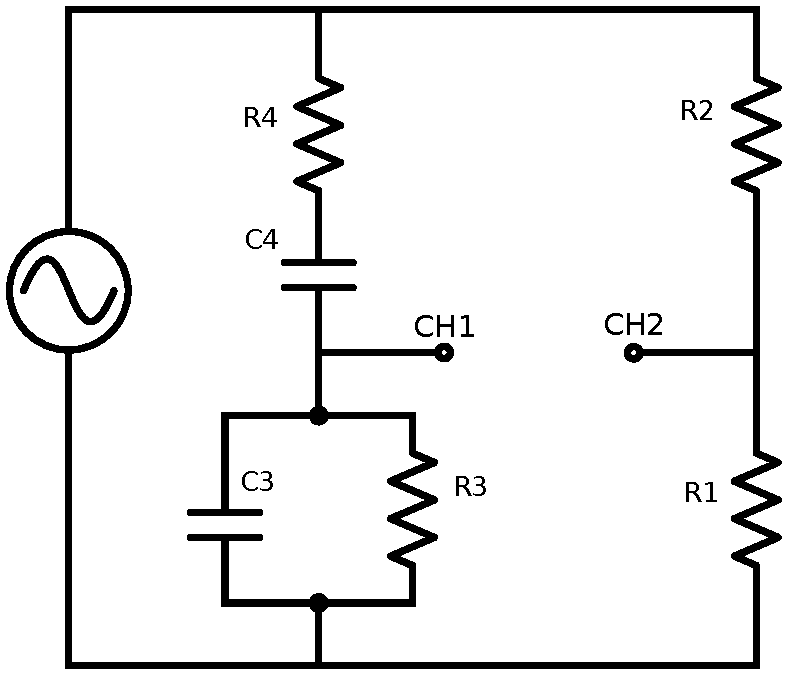
\includegraphics[width=0.30\textwidth]{schema2.pdf}
    \caption{Schema del ponte di Wien invertito}
    \label{fig:Winv}
\end{wrapfigure}

\subsection{Acquisizione e analisi dati}
Utilizzando un ponte di Wien ``invertito'' è possibile creare un filtro notch. Esso non è efficace come quello montato nell'esperienza precedente ma è tuttavia interessante in quanto entrambi i capi del circuito contribuiscono alla creazione del segnale finale. Come si vede in Fig. \ref{fig:Winv}, infatti sia $V_1$ che $V_2$ sono variabili nel tempo. Un'implicazione di ciò è che un eventuale circuito collegato al ponte di Wien non può essere messo a terra (per questo non è stato possibile eseguire direttamente una misura della differenza di potenziale tra i capi attraverso l'oscilloscopio, il quale è per struttura messo a massa).

In questo caso tutte le componenti circuitali sono note ($R_1 = R_2 = R_3 = R_4 \simeq R = (1000 \pm 10)\si{\ohm}$ e $C_1 = C_2 \simeq C = (0.1 \pm 0.05)\si{\micro\farad}$)\footnote{In questo caso abbiamo scelto come incertezza $\delta R$ e $\delta C$ valori tali per cui $R$ e $C$ fossero compatibili con i valori reali delle resistenze e capacità utilizzato.} e ciò che faremo sarà misurare il voltaggio in CH1 e CH2 e rispettiva differenza di fase per diversi valori di frequenza $\nu$. Riportiamo ora le equazioni del circuito ricavate analiticamente: 

\noindent
\begin{minipage}{.5\linewidth}
\begin{equation}
V(CH1) = \left(\frac{V_{in}}{3+i(\omega R C - \frac{1}{\omega R C})}\right)
\label{eq:V1}
\end{equation}
\begin{equation}
V(CH2) = \frac{V_{in}}{2}
\label{eq:V(CH2)}
\end{equation}
\end{minipage}%
\begin{minipage}{.5\linewidth}
\begin{equation}
\varphi_{2|1}=arctan\left[\frac{1}{3 C R \omega}-\frac{C R \omega}{3}\right]
\label{eq:F12}
\end{equation}
\end{minipage}\break

Poichè a noi interessa il valore di tensione a cui il circuito collegato al filtro è sottoposto, dovremo ricavare $V_{out}=V(CH1)-V(CH2)$, da cui segue immediatamente:

\begin{wrapfigure}[10]{r}[0pt]{90mm}
	\centering
    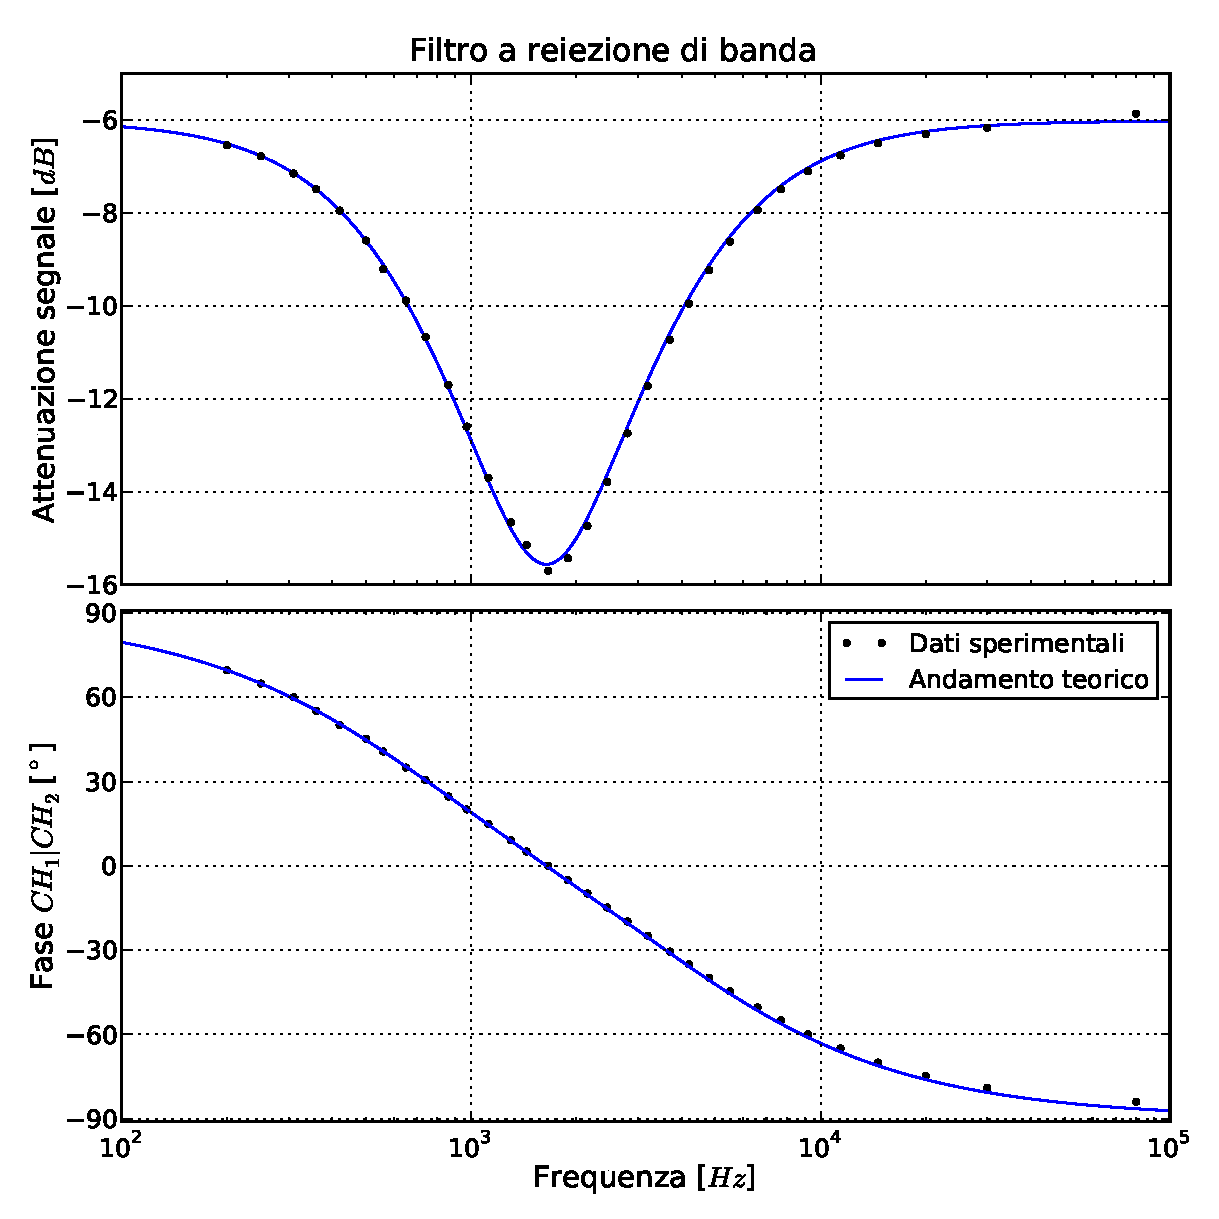
\includegraphics[width=93mm]{notch.pdf}
    \caption{Diagrammi di Bode per il ponte di Wien invertito \phantom {trollolollo} (Notch).}
    \label{fig:notch}
\end{wrapfigure}

\begin{equation}
V_{out}=V_{in} \frac{1}{2} \sqrt{1-\frac{8 C^2 R^2 \omega^2}{C^4 R^4 \omega^4+7 C^2 R^2 \omega^2+1}}
\end{equation}

%usare questa eq nello script python !! phi=arctan[1/2 Sqrt[1 - (8 C^2 R^2 x^2)/(1 + 7 C^2 R^2 x^2 + C^4 R^4 x^4)]]

Come vediamo subito, sia per $\omega \rightarrow \infty$ che per $\omega \rightarrow 0$, $V_{out}=\frac{1}{2}$. Eseguendo una semplice derviata e ponendola uguale a zero, si verifica immediatamente che il valore di massima attenuazione di segnale si ottiene per la frequenza di $\nu_0=\frac{1}{2 \pi R C}$.

Per l'acquisizione dati abbiamo deciso di prendere i dati circa ogni 5 gradi di sfasamento tra i segnali. Ciò è stato fatto sapendo che la scala più opportuna per l'analisi è quella logaritmica su tutti i dati tranne che sugli angoli. \`E dunque una scelta saggia basarsi sugli angoli per decidere un metodo di lavoro.

I dati rilevati sono riportati nel grafico in Fig \ref{fig:notch}. Come vediamo nel primo grafico, il valore per $\nu=0$ è circa $-6 \si{\decibel}$. Imponendo la condizione $-6=20Log_{10}(\frac{V_{out}}{V_{in}})$, si ottiene subito la relazione $V_{out} \approx \frac{1}{2} V_{in}$. Notiamo come l'attenuazione di segnale non superi i $16 \si{\decibel}$. Se lo paragoniamo al filtro notch costruito utilizzando condensatore ed induttanza vediamo subito che il ponte di Wien non è così efficace (eravamo infatti arrivati a -30/-40dB).\\